\documentclass[10pt,slovak,a4paper]{article}

\usepackage[slovak]{babel}
\usepackage[IL2]{fontenc} 
\usepackage[utf8]{inputenc}
\usepackage{graphicx}
\usepackage{url}
\usepackage{hyperref}
\usepackage{cite}
\usepackage{amsmath}

\pagestyle{headings}

\title{Algoritmy odporúčania filmov v Netflix\thanks{Semestrálny projekt v predmete Metódy inžinierskej práce, ak. rok 2024/25, vedenie: Ing. Richard Marko, PhD}}

\author{Yehor Bohuslavskyi\\[2pt]
	{\small Slovenská technická univerzita v Bratislave}\\
	{\small Fakulta informatiky a informačných technológií}\\
	{\small \texttt{xbohuslavkyi@stuba.sk}}
	}

\date{\small 17. oktober 2024}

\begin{document}

\begin{figure}[h!]
  \centering
  
\includegraphics[width=\textwidth]{Images/fiit_logo.png} 
\end{figure}

\maketitle

\begin{abstract}
Túto tému som si vybral, pretože je veľmi zaujímavé, ako technológie a umelá inteligencia(ktorá je v súčasnosti jednou z najrozvíjajúcejších sa tém) ovplyvňujú naše každodenné rozhodovanie o tom, čo sledujeme. Ja som zvedavý, že ako po zhliadnutí jedného tureckého filmu, ktorý som ani neohodnotil, sa mi v odporúčaniach začali objavovať podobné filmy. 

V systéme sa nachádza viac, ako 15 000 filmov a zobrazuje vám len tie, ktoré sa vám budú páčiť (neskôr dozvieme sa, ako to funguje). Fakt: ani jeden používateľ Netflix nebol by schopný si samostatne nájsť film alebo seriál, ktorý by sa mu páčil bez požívania algoritmu odporúčania filmov \cite{Netflix:Algorithm}.
 
V tomto článku sa podrobne pozrieme na algoritmy spoločnosti Netflix. V súčasnosti je systém Netflix postavený na algoritme, ktorý využíva umelú inteligenciu a strojové učenie. Pozrieme sa aj na umiestnenie odporúčaní na obrazovke, kde je niekoľko typov návrhov. Prvým je „Odporúčané pre vás“, po ňom idú „Trendy“, na stránke sa nachádza aj záložka „New Releases“\cite{Netflix:Recommendation:System}.

Podrobne sa pozrieme aj na filtračné algoritmy, ktoré sa delia na dva hlavné typy. Akú rolu odohrávajú hodnotenia a správania používateľov v rámci algoritmu collaborative filtering a „filtrovanie na základe obsahu“.

Zaujímavým aspektom sú aj systémy hodnotenia. Patrí medzi ne „Personalizované hodnotenie videa (PVR)“, „Top-N Ranking“, „Rebríček obľúbených filmov“ a „Zoznam zaujímavého obsahu na neskoršie sledovanie“. Každé z týchto hodnotení je personalizované pre jednotlivých používateľov, čo je veľmi zaujímavé.

V rámci článku sa budeme venovať aj typom údajov, ktoré Netflix používa. Tie sa zhruba delia na dva typy: základné typy zhromažďovaných údajov a dodatočné informácie. Medzi základné patria „interakcie používateľa so stránkou“, ktoré pozostávajú z histórie sledovania a hodnotení. Druhým typom sú „korelačné údaje“, „informácie o obsahu knižnice Netflix“, ako napríklad žánre. Ďalšie uvidíme ako ovplyvňujú  špecifickejšie typy informácií, ako sú napríklad denný čas, používané zariadenie alebo priemerná dĺžka sledovania.

\end{abstract}

\section{Úvod}
Cieľom spoločnosti Netflix je používať odporúčacie algoritmy na maximalizáciu spokojnosti
používateľov. Hlavným cieľom je prispôsobiť obsah každému jednotlivému používateľovi.

Netflix má obrovskú knižnicu obsahu a obmedzené rozhranie obrazovky, čo veľmi sťažuje odporúčanie relevantného obsahu, a každý používateľ má iný vkus, preferencie a zvyky pri sledovaní, takže personalizácia musí byť veľmi presná.\cite{Bennett}
Čo robí Netflix na dosiahnutie tohto cieľa, sa dozviete po tomto článku.

\section{Technológie a Umelá inteligencia v Netflix}
V súčasnosti veľké spoločnosti v IT priemysle využívajú umelú inteligenciu, čo nezostalo bez povšimnutia spoločnosti Netflix, ktorá kombinuje niekoľko modelov a prístupov (tzv. ensemble learning) na vytvorenie najlepších odporúčaní.\cite{Bennett}

\section{Typy Odporúčaní na Netflix}
Netflix používa dvoj úrovňový systém hodnotenia založený na riadkoch, čo to znamená? Obsah je hodnotený dvakrát, v stĺpcoch a v každom riadku, ako sa dozviete v článku ďalej.
Na základe kombinácie týchto prístupov sa vytvárajú personalizované odporúčania pre konkrétneho používateľa.\cite{Habr}

\begin{figure}[h!]
  \centering
  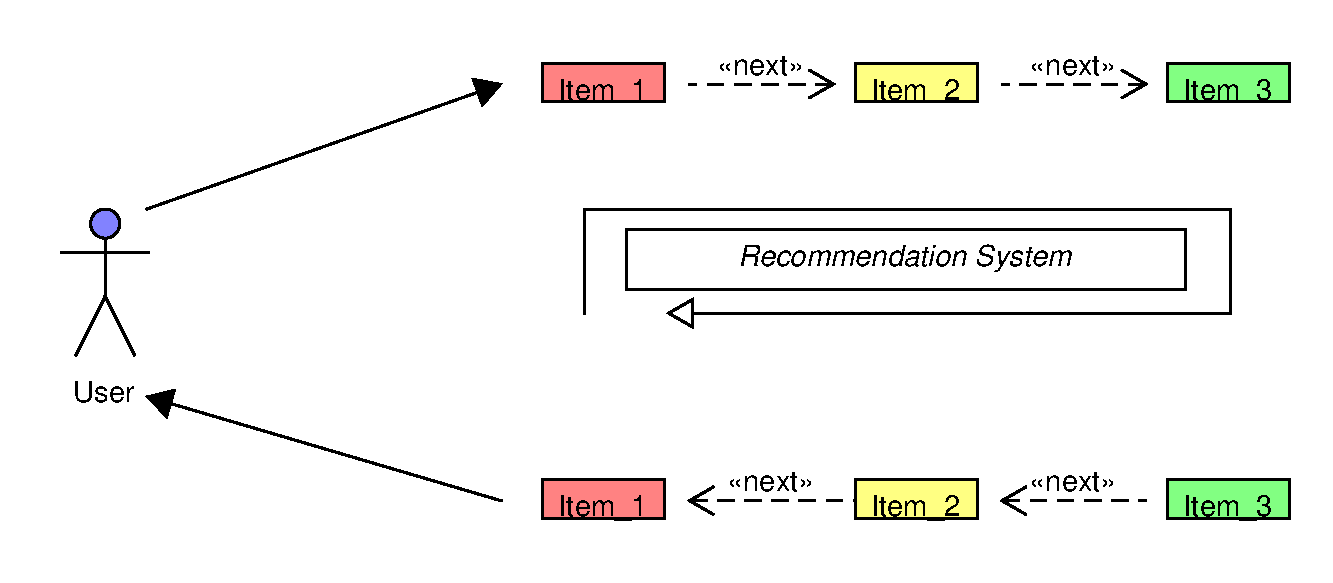
\includegraphics[width=1\textwidth]{Images/RecommendationSystem_pdf.pdf} % Adjust width as needed
  \caption{Recommendation System}
\end{figure}

\section{Filtračné algoritmy}
Netflix používa dva typy filtrovania: kolaboratívne filtrovanie a filtrovanie podľa obsahu. Rozdiel môžete rozoznať podľa názvu, ale poďme sa naň pozrieť bližšie.  

Kolaboratívne filtrovanie je algoritmus, ktorý pomáha odhadnúť záujmy nového používateľa na základe akcií predchádzajúcich členov cieľového publika, rozdeľuje používateľov podľa zadaných charakteristík. Najprv identifikuje podobné záujmy a potom hľadá podobné skóre. Každý používateľ dostane takzvanú váhu. Keď sa váha niekoľkých návštevníkov stane maximálne podobnou, sú spojení do skupiny „susedov“ a zobrazí sa im rovnaký obsah.\cite{Collaborative:Filtering}

Filtrovanie na základe obsahu zohľadňuje pri odporúčaní vlastnosti položky a preferencie používateľa. Tento prístup zahŕňa analýzu samotného obsahu, napríklad filmových žánrov, hercov alebo kľúčových slov, a jeho porovnanie s predchádzajúcimi preferenciami používateľov.\cite{Linkedin}



\begin{figure}[h!]
  \centering
  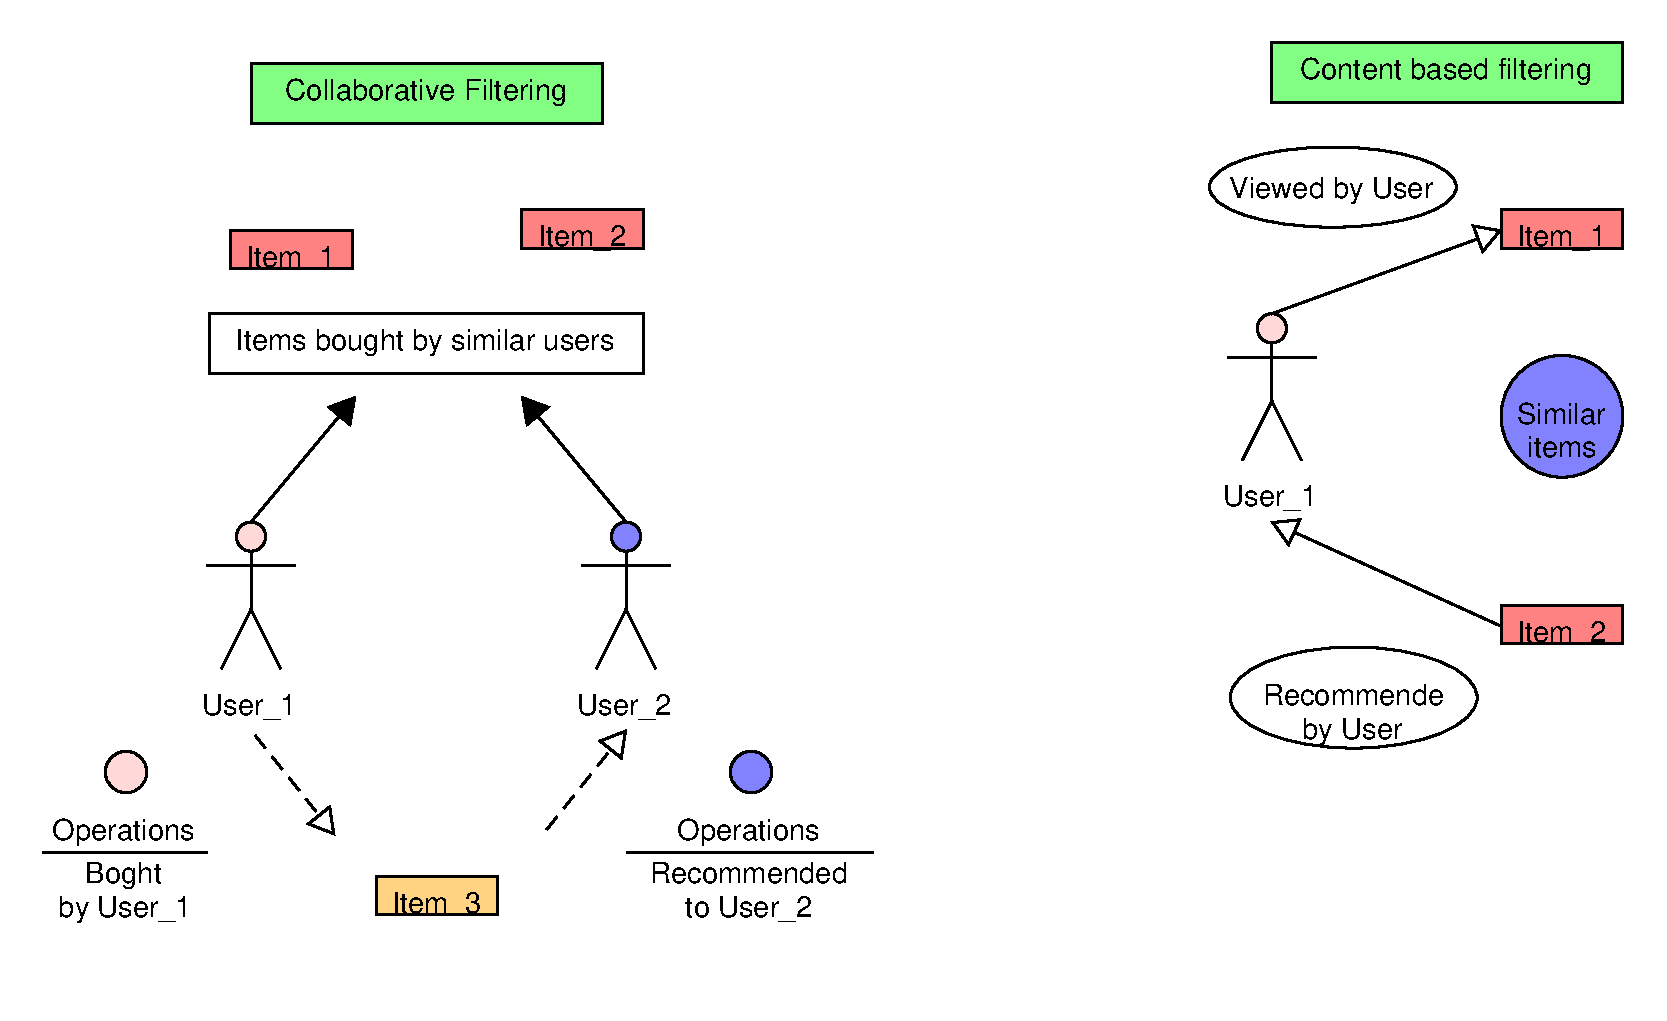
\includegraphics[width=1\textwidth]{Images/Filtering_pdf.pdf} % Adjust width as needed
  \caption{Type of Filtering}
\end{figure}

\section{Systémy Hodnotenia}
 Kľúčovými zložkami odporúčacieho systému spoločnosti Netflix je niekoľko personalizovaných systémov hodnotenia, z ktorých každý je navrhnutý tak, aby zohľadňoval rôzne aspekty zvykov používateľa pri sledovaní. Poďme sa do týchto systémov ponoriť a preskúmať, ako fungujú.

Personalizovaný rebríček videí (PVR) je jedným z najsofistikovanejších nástrojov spoločnosti Netflix a neustále sa prispôsobuje na základe spätnej väzby používateľov. Tento model založený na hlbokom učení využíva historické údaje o zvykoch používateľa pri sledovaní na uprednostňovanie obsahu, ktorý ho pravdepodobne najviac zaujíma. Sila PVR spočíva v jeho schopnosti nielen pochopiť minulé správanie, ale aj predpovedať budúce interakcie.\cite{Argoid}\cite{Data}

Systém Top-N Ranking - ako už názov napovedá, tento model generuje zoznam N najlepších odporúčaní obsahu pre každého používateľa. Robí to kombináciou kolaboratívneho a obsahového filtrovania. Obsah je zoradený na základe toho, ako dobre zodpovedá preferenciám používateľa, čím sa zabezpečí, aby sa najrelevantnejšie tituly zobrazovali na vrchole obrazovky.\cite{Top}


Poradie obľúbených filmov je ďalší model hodnotenia, ktorý využíva trendový obsah. Netflix používa tento systém na zaraďovanie filmov na základe ich celosvetovej aj regionálnej popularity. Ukážkovým príkladom bolo obdobie pandémie COVID-19, keď prudko stúpol počet divákov filmu Nákaza.\cite{Top} 


Zaraďovanie zaujímavého obsahu na neskoršie pozretie
Netflix používa aj systém hodnotenia, ktorý sa zameriava na zaujímavý obsah, ktorý si používatelia môžu chcieť pozrieť neskôr. Sledovaním tohto správania Netflix zabezpečuje, aby platforma zostala relevantná pre široký vkus používateľov a aby sa mohli vždy vrátiť k predtým sledovanému obsahu.\cite{Top}\cite{Ranking:System}


Netflix sa neustále zlepšuje prostredníctvom A/B testovania. Netflix pravidelne testuje varianty svojich odporúčacích algoritmov na rôznych skupinách používateľov a analyzuje, ktoré modely vedú k vyššej angažovanosti a spokojnosti.\cite{Ranking:System}

\section{Typy Údajov v Netflix}
Cesta spoločnosti Netflix k personalizácii sa začína zberom údajov. A nejde len o to, aké seriály sa vám páčia. Netflix analyzuje všetko od žánrov, ktoré preferujete, až po režisérov, ktorých sledujete, dĺžku sledovania a dennú dobu. Nie je to len súbor údajov - je to základom schopnosti spoločnosti Netflix prispôsobiť váš zážitok zo sledovania. Vďaka viac ako 1 300 klastrom odporúčaní Netflix vie nielen to, že máte radi thrillery; vie, že máte radi psychologické thrillery so silnými ženskými hrdinkami, ktoré sledujete väčšinou cez víkend večer.\cite{Bennett}\cite{Data}

\section{Záver}
Odporúčací systém Netflix je zložitý mechanizmus na spracovanie veľkého množstva údajov a preferencií používateľov. Je to kľúčový nástroj na udržanie záujmu používateľov a na to, aby sa nestratili v obrovskej knižnici obsahu.

\bibliography{literatura}
\bibliographystyle{plain}

\end{document}
